\documentclass[article,shortnames]{jss}
\usepackage{amsmath}
\usepackage{amsfonts}
\usepackage{amssymb}
\usepackage{graphicx}
\usepackage{algorithm}
\usepackage[latin1]{inputenc}
\usepackage[T1]{fontenc}
\usepackage{fancyhdr}
\usepackage{subfigure}
\usepackage{epstopdf}
\usepackage{hyperref}
\usepackage{fancybox}
\usepackage{tikz}
\usepackage{listings}

\usepackage{lmodern}

\usetikzlibrary{arrows}
\newtheorem{theorem}{Theorem}
\newtheorem{acknowledgement}[theorem]{Acknowledgement}
\newtheorem{axiom}[theorem]{Axiom}
\newtheorem{case}[theorem]{Case}
\newtheorem{claim}[theorem]{Claim}
\newtheorem{conclusion}[theorem]{Conclusion}
\newtheorem{condition}[theorem]{Condition}
\newtheorem{conjecture}[theorem]{Conjecture}
\newtheorem{corollary}[theorem]{Corollary}
\newtheorem{criterion}[theorem]{Criterion}
\newtheorem{definition}[theorem]{Definition}
\newtheorem{example}[theorem]{Example}
\newtheorem{exercise}[theorem]{Exercise}
\newtheorem{lemma}[theorem]{Lemma}
\newtheorem{notation}[theorem]{Notation}
\newtheorem{problem}[theorem]{Problem}
\newtheorem{proposition}[theorem]{Proposition}
\newtheorem{remark}[theorem]{Remark}
\newtheorem{solution}[theorem]{Solution}
\newtheorem{summary}[theorem]{Summary}


\newcommand{\BiiPS}{\pkg{BiiPS}}
\newcommand{\JAGS}{\pkg{JAGS}}
\newcommand{\rjags}{\pkg{rjags}}
\newcommand{\BUGS}{\proglang{BUGS}}
\newcommand{\OpenBUGS}{\pkg{OpenBUGS}}
\newcommand{\WinBUGS}{\pkg{WinBUGS}}
\newcommand{\Stan}{\pkg{Stan}}
\newcommand{\R}{\proglang{R}}
\newcommand{\Cpp}{\proglang{C++}}
\newcommand{\Matlab}{\proglang{Matlab}}
\newcommand{\CODA}{\pkg{coda}}


\newcommand{\Norm}{\mathcal{N}}

%%%%%%%%%%%%%%%%%%%%%%%%%%%%%%%%%%%%%%%%
%%%%%%%% Listings stuff
%%%%%%%%%%%%%%%%%%%%%%%%%%%%%%%%%%%%%%%%

\lstloadlanguages{R,Matlab}
\definecolor{mygreen}{rgb}{0,0.6,0}
\definecolor{mygray}{rgb}{0.5,0.5,0.5}
\definecolor{mymauve}{rgb}{0.58,0,0.82}
\definecolor{shadecolor}{rgb}{0.9,0.9,0.9}
\definecolor{darkblue}{rgb}{0,0,.5}
\definecolor{darkgreen}{rgb}{0,0.5,0}

%\renewcommand{\ttdefault}{pcr}

% Define Matbiips style
\lstdefinestyle{matbiips}{
  backgroundcolor=\color{shadecolor},   % choose the background color; you must add \usepackage{color} or \usepackage{xcolor}
  basicstyle=\scriptsize\ttfamily,        % the size of the fonts that are used for the code
  breakatwhitespace=false,         % sets if automatic breaks should only happen at whitespace
  breaklines=true,                 % sets automatic line breaking
  captionpos=t,                    % sets the caption-position to bottom
  commentstyle=\color{mygreen},    % comment style
  deletekeywords={mean},            % if you want to delete keywords from the given language
  escapeinside={\%*}{*)},          % if you want to add LaTeX within your code
  extendedchars=true,              % lets you use non-ASCII characters; for 8-bits encodings only, does not work with UTF-8
  frame=none,                    % adds a frame around the code
  keepspaces=true,                 % keeps spaces in text, useful for keeping indentation of code (possibly needs columns=flexible)
  keywordstyle=\color{blue},       % Common Matlab keyword style
  keywordstyle=[2]\color{blue}\bfseries,
  language=Matlab,                 % the language of the code
  morekeywords={},            % if you want to add more keywords to the set
  morekeywords=[2]{biips_pimh_update,biips_summary,biips_pimh_samples,biips_model},
  numbers=none,                    % where to put the line-numbers; possible values are (none, left, right)
  numbersep=5pt,                   % how far the line-numbers are from the code
  numberstyle=\tiny\color{mygray}, % the style that is used for the line-numbers
  rulecolor=\color{black},         % if not set, the frame-color may be changed on line-breaks within not-black text (e.g. comments (green here))
  showspaces=false,                % show spaces everywhere adding particular underscores; it overrides 'showstringspaces'
  showstringspaces=false,          % underline spaces within strings only
  showtabs=false,                  % show tabs within strings adding particular underscores
  stepnumber=2,                    % the step between two line-numbers. If it's 1, each line will be numbered
  stringstyle=\color{mymauve},     % string literal style
  tabsize=2,                       % sets default tabsize to 2 spaces
  title={\tiny Matbiips},                   % show the filename of files included with \lstinputlisting; also try caption instead of title
  %emph=[1]{biips_pimh_update,biips_summary,biips_pimh_samples,biips_model},emphstyle=[1]\color{blue}\textbf,
}

% Define Rbiips style
\lstdefinestyle{Rbiips}{
  language=R,                % the language of the code
  basicstyle=\scriptsize\ttfamily,           % the size of the fonts that are used for the code
  numbers=none,                   % where to put the line-numbers
  numberstyle=\tiny\color{gray},  % the style that is used for the line-numbers
  stepnumber=2,                   % the step between two line-numbers. If it's 1, each line
                                  % will be numbered
  numbersep=5pt,                  % how far the line-numbers are from the code
  backgroundcolor=\color{white},      % choose the background color. You must add \usepackage{color}
  showspaces=false,               % show spaces adding particular underscores
  showstringspaces=false,         % underline spaces within strings
  showtabs=false,                 % show tabs within strings adding particular underscores
  frame=none,                   % adds a frame around the code
  rulecolor=\color{black},        % if not set, the frame-color may be changed on line-breaks within not-black text (e.g. commens (green here))
  tabsize=2,                      % sets default tabsize to 2 spaces
  captionpos=t,                   % sets the caption-position to bottom
  breaklines=true,                % sets automatic line breaking
  breakatwhitespace=false,        % sets if automatic breaks should only happen at whitespace
  title={\tiny \color{gray} Rbiips},                   % show the filename of files included with \lstinputlisting;
                                  % also try caption instead of title
  keywordstyle=\color{blue},          % keyword style
  commentstyle=\color{darkgreen},       % comment style
  stringstyle=\color{mymauve},         % string literal style
  escapeinside={\%*}{*)},            % if you want to add a comment within your code
  morekeywords={}               % if you want to add more keywords to the set 
  }
  % DEFINE BUGS STYLE
\lstdefinestyle{bugs}{
  basicstyle=\scriptsize\ttfamily,           % the size of the fonts that are used for the code
  numbers=none,                   % where to put the line-numbers
  numberstyle=\tiny\color{gray},  % the style that is used for the line-numbers
  stepnumber=2,                   % the step between two line-numbers. If it's 1, each line
                                  % will be numbered
  numbersep=5pt,                  % how far the line-numbers are from the code
  backgroundcolor=\color{shadecolor},      % choose the background color. You must add \usepackage{color}
  showspaces=false,               % show spaces adding particular underscores
  showstringspaces=false,         % underline spaces within strings
  showtabs=false,                 % show tabs within strings adding particular underscores
  frame=none,                   % adds a frame around the code
  rulecolor=\color{black},        % if not set, the frame-color may be changed on line-breaks within not-black text (e.g. commens (green here))
  tabsize=2,                      % sets default tabsize to 2 spaces
  captionpos=t,                   % sets the caption-position to bottom
  breaklines=true,                % sets automatic line breaking
  breakatwhitespace=false,        % sets if automatic breaks should only happen at whitespace
  title={\tiny \lstname },                   % show the filename of files included with \lstinputlisting;
                                  % also try caption instead of title
  keywordstyle=\color{blue},          % keyword style
  keywordstyle=[2]\color{blue}\bfseries,          % keyword style 2
  commentstyle=\color{darkgreen},       % comment style
  stringstyle=\color{mymauve},         % string literal style
  escapeinside={\%*}{*)},            % if you want to add a comment within your code
  morekeywords={dnorm,dgamma,dcat,for, <-},               % if you want to add more keywords to the set
  morekeywords=[2]{model, data,var}               % if you want to add more keywords to the set
  }

%%%%%%%%%%%%%%%%%%%%%%%%%%%%%%%%%%%%%%%%
%%%%%%%% TIKZ stuff
%%%%%%%%%%%%%%%%%%%%%%%%%%%%%%%%%%%%%%%%

\tikzstyle{every node}=[font=\footnotesize]

\tikzstyle{state}=[circle,
                                    thick,
                                    minimum size=.1cm,
                                    draw=blue!80,
                                    fill=blue!20
                                    ]

% The measurement vector is represented by an orange circle.
\tikzstyle{measurement}=[circle,
                                                thick,
                                                minimum size=.1cm,
                                                draw=orange!80,
                                                fill=orange!25]

\tikzstyle{input}=[rectangle, rounded corners,
                                    thick,
                                    text width=3cm,
                                    draw=blue!80,
                                    fill=blue!20,
                                    text centered,
                                    font=\large,
                                    ]
\tikzstyle{processing}=[rectangle, rounded corners,
                                    thick,
                                    text width=3cm,
                                    draw=green!80,
                                    fill=green!20,
                                    text centered,
                                    font=\large,
                                    ]
\tikzstyle{output}=[rectangle, rounded corners,
                                                thick,
                                                text width=3cm,
                                                draw=orange!80,
                                                fill=orange!25,
                                                text centered,
                                    font=\large,]

%%%%%%%%%%%%%%%%%%%%%%%%%%%%%%%%%%%%%%%%%%%
%%%%%%%% END OF TIKZ STUFF
%%%%%%%%%%%%%%%%%%%%%%%%%%%%%%%%%%%%%%%%%%%


%%%%%%%%%%%%%%%%%%%%%%%%%%%%%%
%% declarations for jss.cls %%%%%%%%%%%%%%%%%%%%%%%%%%%%%%%%%%%%%%%%%%
%%%%%%%%%%%%%%%%%%%%%%%%%%%%%%

%% almost as usual
\author{A. Todeschini\\INRIA\And
        M. Fuentes\\INRIA\And
        F. Caron\\Univ. of Oxford\And
        P. Legrand\\Univ. of Bordeaux\And
        P. Del Moral\\UNSW
        }
\title{\BiiPS: Bayesian Inference with Interacting Particle Systems}

%% for pretty printing and a nice hypersummary also set:
\Plainauthor{A. Todeschini, M. Fuentes, F. Caron, P. Legrand, P. Del Moral} %% comma-separated
\Plaintitle{BiiPS: Bayesian Inference with Interacting Particle Systems} %% without formatting
\Shorttitle{\BiiPS} %% a short title (if necessary)

%% an abstract and keywords
\Abstract{
  The abstract of the article.
}
\Keywords{Sequential Monte Carlo, Markov Chain Monte Carlo, particle MCMC, graphical models, \BUGS, \JAGS, \Cpp, \R, \Matlab}
\Plainkeywords{Sequential Monte Carlo, Markov Chain Monte Carlo, particle MCMC, graphical models, BUGS, JAGS, C++, R, Matlab} %% without formatting
%% at least one keyword must be supplied

%% publication information
%% NOTE: Typically, this can be left commented and will be filled out by the technical editor
%% \Volume{50}
%% \Issue{9}
%% \Month{June}
%% \Year{2012}
%% \Submitdate{2012-06-04}
%% \Acceptdate{2012-06-04}

%% The address of (at least) one author should be given
%% in the following format:
\Address{
  Adrien Todeschini\\
  INRIA Bordeaux Sud-Ouest\\
  200 avenue de la vieille tour\\
  33405 Talence Cedex, France
  E-mail: \email{Adrien.Todeschini@inria.fr}\\
  URL: \url{https://sites.google.com/site/adrientodeschini/}
}
%% It is also possible to add a telephone and fax number
%% before the e-mail in the following format:
%% Telephone: +43/512/507-7103
%% Fax: +43/512/507-2851

%% for those who use Sweave please include the following line (with % symbols):
%% need no \usepackage{Sweave.sty}

%% end of declarations %%%%%%%%%%%%%%%%%%%%%%%%%%%%%%%%%%%%%%%%%%%%%%%


\begin{document}

%% include your article here, just as usual
%% Note that you should use the \pkg{}, \proglang{} and \code{} commands.

%\section[About Java]{About \proglang{Java}}
%% Note: If there is markup in \(sub)section, then it has to be escape as above.

\section{Introduction}
Bayesian inference consists in approximating the conditional probability law of an unknown parameter $X$ given some observations $Y$. Several problems such as signal filtering or clustering can be cast into this framework. This conditional probability law is in general not analytically tractable. Markov Chain Monte Carlo (MCMC) methods~\citep{Gilks1995,Robert2004} have been used over the past 20 years in order to provide samples asymptotically distributed from the conditional distribution of interest.
As stated by~\cite{Cappe2000}
\begin{quote}
%\begin{textit}
\textit{``The main factor in the success of MCMC algorithms is that they can be implemented with little effort in a large variety of settings. This is obviously true of the Gibbs sampler, which, provided some conditional distributions are available, simply runs by generating from these conditions, as shown by the BUGS software.''}
%\end{textit}
\end{quote}

The \BUGS (which stands for Bayesian Inference Using Gibbs Sampling) software has actually greatly contributed to the development of Bayesian and MCMC techniques among applied fields~\citep{Lunn2012}. \BUGS\ allows the user to define statistical models in a natural language, the \BUGS\ language~\citep{Gilks1994}, then evaluates the posterior distribution of the parameter $X$ given the data using MCMC methods and provides some summary statistics. It is easy to use even for people not aware of MCMC methods and works as a black box. Various software have been developed based on or inspired by the \BUGS\ software, such as \WinBUGS, \OpenBUGS, \JAGS\ or \Stan.

A new generation of algorithms, based on interacting particle systems, has appeared over the last 15 years. Those methods are known under the names of \textit{interacting MCMC, particle filtering, sequential Monte Carlo methods}, etc. For some problems, those methods have shown to be more appropriate than MCMC methods, in particular for time series or highly correlated variables~\citep{Doucet2000,Doucet2001,Liu2001,DelMoral2004}. Contrary to MCMC methods, those methods do not require the convergence of the algorithm to some equilibrium and are particularly suited to dynamical estimation problems such as signal filtering or target tracking.

Traditionally, those methods have been restricted to the class of state-space models or hidden Markov Chain models for which those models are particularly suited~\citep{Cappe2005}. However, SMC methods have been used outside of this framework, either alone~\citep{Fearnhead2004,Fearnhead2007,Caron2008,Caron2012}, or within a MCMC algorithm~\citep{Andrieu2010}.

Describe general objectives of the BiiPS Software: build on the \BUGS\ language for describing complex statistical models and runs SMC and particle MCMC algorithms as a black box. It provides interfaces with the statistical software \R\ and \Matlab\. GPL, etc...

This article is organized as follows. Section~\ref{sec:graphical} describes the representation of the statistical model as a graphical model and the BUGS language. Section~\ref{sec:SMC} provides the basics of SMC and particle MCMC algorithms. The main features of the \BiiPS\ software and its interfaces to \R\ and \Matlab\ are given in Section~\ref{sec:biips}. Section~\ref{sec:examples} provides several examples of the use of the software. In Section~\ref{sec:discussion} we discuss the relative merits and limits of \BiiPS\ compared to alternatives.

\section{Graphical Models and BUGS language}
\label{sec:graphical}

\subsection{Graphical models}
A statistical model is represented by a joint distribution $\mathcal{L}(X,Y)$ over the parameters $X$ and the observations $Y$. The joint distribution decomposes as $\mathcal{L}(X,Y)=\mathcal{L}(Y|X)\mathcal{L}(X)$ where the two terms of the right-hand side are respectively named \textit{likelihood} and \textit{prior}. As stated above, the objective of Bayesian Inference is to approximate the posterior distribution $\mathcal{L}(X|Y=y)$ after having observed some data $y$.

A convenient way of representing a statistical model is through a directed acyclic graph~\citep{Lauritzen1996,Green2003,Jordan2004}. Such a graph provides at a glance the conditional independencies between variables and displays the decomposition of the joint distribution. An example of graph is given in Figure~\ref{fig:graph}.


*** PROVIDE SOME EXAMPLES, hmm and another ***


\begin{figure}[h!]
\begin{center}
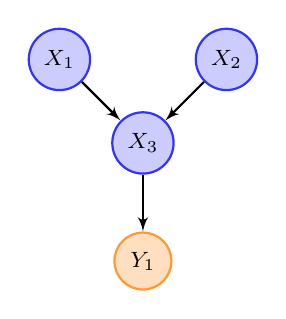
\begin{tikzpicture}[node distance=1.5cm,auto,>=latex']
\node (X_3)   [state] {$X_3$};
\node (X_2)   [state,above right of=X_3] {$X_{2}$};
\node (X_1)   [state,above left of=X_3] {$X_1$};
\node (Y_1)   [measurement,below of=X_3] {$Y_1$};
 \path[->] (X_1) edge[thick] (X_3);
 \path[->] (X_2) edge[thick] (X_3);
 \path[->] (X_3) edge[thick] (Y_1);
 \end{tikzpicture}
 \caption{Example of a Graphical model. An arrow from node $A$ to node $B$ indicates that ``$A$ is a parent of $B$''. Let $Z=(X,Y)$ and $n$ the number of elements in $Z$. Then the joint distribution decomposes as $\pi(z)=\prod_{i=1}^n \pi(z_i|\text{pa}(z_i))$ where $\text{pa}(z_i)$ is the set of parents of node $Z_i$. In the example, the joint distribution decomposes as $\pi(x_1,x_2,x_3,y_1)=\pi(x_1)\pi(x_2)\pi(x_3|x_1,x_2)\pi(y_1|x_3)$. }
 \label{fig:graph}
 \end{center}
 \end{figure}

%\bigskip\noindent\shadowbox{\begin{minipage}{4.8in}
\begin{example}{Hidden Markov Model}
\vskip .05in \hrule\vskip .1in
Consider the following model known as an hidden Markov Model, or dynamic model, where we have the following decomposition of the joint distribution of $(X,Y)=(X_1,\ldots,X_n,Y_1,\ldots,Y_n)$
$$
\pi(x,y)=\pi(x_1)\pi(y_1|x_1)\prod_{t=2}^{n}\left [\pi(x_t|x_{t-1})\pi(y_t|x_{t})\right ]
$$
The model can be represented as the directed acyclic graph in Figure~\ref{fig:hmm}.
\end{example}
%\end{minipage} }\bigskip

\begin{figure}[h!]
\begin{center}
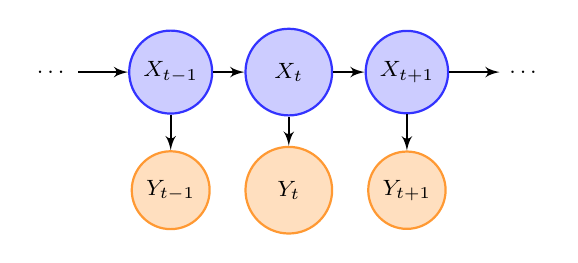
\begin{tikzpicture}[node distance=1.5cm,auto,>=latex']
\node (X_t-2)   [] {\ldots};
\node (X_t-1)   [state,right of=X_t-2] {$X_{t-1}$};
\node (X_t)   [state,minimum size=1.1cm,right of=X_t-1] {$X_t$};
\node (X_t+1)   [state,right of=X_t] {$X_{t+1}$};
\node (X_t+2)   [right of=X_t+1] {\ldots};
 \node (Y_t)   [measurement,minimum size=1.1cm,below of=X_t] {$Y_t$};
 \node (Y_t-1)   [measurement,below of=X_t-1] {$Y_{t-1}$};
 \node (Y_t+1)   [measurement,below of=X_t+1] {$Y_{t+1}$};
 \path[->] (X_t-1) edge[thick] (X_t);
 \path[->] (X_t-2) edge[thick] (X_t-1);
 \path[->] (X_t) edge[thick] (X_t+1);
 \path[->] (X_t+1) edge[thick] (X_t+2);
 \path[->] (X_t) edge[thick] (Y_t);
 \path[->] (X_t-1) edge[thick] (Y_t-1);
 \path[->] (X_t+1) edge[thick] (Y_t+1);
 \end{tikzpicture}
 \caption{Graphical representation of a hidden Markov Model as a directed acyclic graph.}
 \label{fig:hmm}
 \end{center}
 \end{figure}

\subsection{BUGS language}

Description of the BUGS language, and example with the HMM and another example

Consider the following Gaussian HMM model
\begin{align}
\pi(x_1)&=\Norm (x_1;mu_0,1/\lambda_0)\\
\pi(x_t|x_{t-1})&=\Norm (x_t;x_{t-1},1/\lambda_x)\\
\pi(y_t|x_{t})&=\Norm (y_t;x_{t},1/\lambda_y)
\end{align}
where $\Norm(x;m,\sigma^2)$ denotes the Gaussian pdf of mean m and variance $\sigma^2$ evaluated at $x$.


\begin{example}{HMM in BUGS language}
\code{\\
var x[t_max] y[t_max]\\
model\\
\{\\
\qquad  x[1] ~ dnorm(mu_0, lambda_0)\\
  y[1] ~ dnorm(x[1], lambda_y)\\
  for (t in 2:t_max)\\
  \{\\
    x[t] ~ dnorm(x[t-1], lambda_x)\\
    y[t] ~ dnorm(x[t], lambda_y)\\
  \}\\
\}\\
}
\end{example}





\section{Sequential Monte Carlo methods}
\label{sec:SMC}
\subsection{Reordering of the graphical model}
For later notational convenience, a graphical model will be rearranged in the following manner.
\begin{enumerate}
\item Sort the nodes of the graphical model according to a topological order (node after all his parents), by giving priority to measurement nodes compared to state nodes (the sort is not unique)
\item Group successive measurement or state nodes
\item We then obtain an ordering $(X_1,Y_1,X_2,Y_2,\ldots,X_n,Y_n)$
\end{enumerate}
Figure \ref{fig:graphorder} gives an example of rearrangement of a graphical model.

\begin{figure}[h!]
\begin{center}
\subfigure[Graphical model before rearrangement]{
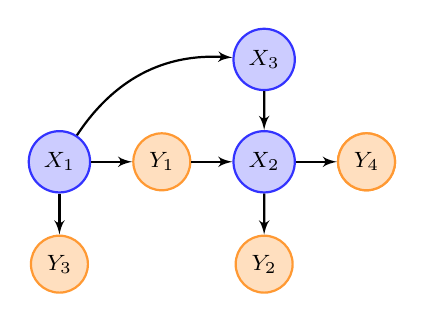
\begin{tikzpicture}[node distance=1.3cm,auto,>=latex',scale=.2]
\node (X_1)   [state] {$X_1$};
\node (Y_1)   [measurement,right of=X_1] {$Y_{1}$};
\node (X_2)   [state,right of=Y_1] {$X_2$};
\node (Y_4)   [measurement,right of=X_2] {$Y_4$};
\node (Y_3)   [measurement,below of=X_1] {$Y_3$};
 \node (X_3)   [state,above of=X_2] {$X_3$};
 \node (Y_4)   [measurement,right of=X_2] {$Y_{4}$};
 \node (Y_2)   [measurement,below of=X_2] {$Y_2$};
 \path[->] (X_1) edge[thick] (Y_3);
 \path[->] (X_1) edge[thick,style={bend left}] (X_3);
 \path[->] (X_1) edge[thick] (Y_1);
 \path[->] (Y_1) edge[thick] (X_2);
 \path[->] (X_3) edge[thick] (X_2);
 \path[->] (X_2) edge[thick] (Y_2);
 \path[->] (X_2) edge[thick] (Y_4);
 \end{tikzpicture}}\hskip 1cm
 \subfigure[Topological sort (with priority to measurement nodes): $(X_1,Y_1,Y_3,X_3,X_2,Y_4,Y_2)$]{
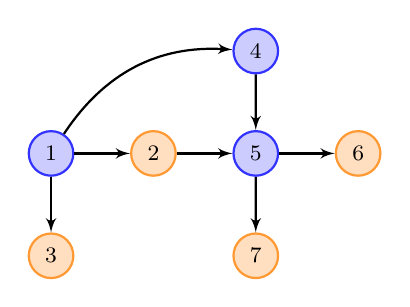
\begin{tikzpicture}[node distance=1.3cm,auto,>=latex',scale=.2]
\node (X_1)   [state] {1};
\node (Y_1)   [measurement,right of=X_1] {2};
\node (X_2)   [state,right of=Y_1] {5};
\node (Y_3)   [measurement,below of=X_1] {3};
 \node (X_3)   [state,above of=X_2] {4};
 \node (Y_4)   [measurement,right of=X_2] {6};
 \node (Y_2)   [measurement,below of=X_2] {7};
 \path[->] (X_1) edge[thick] (Y_3);
 \path[->] (X_1) edge[thick,style={bend left}] (X_3);
 \path[->] (X_1) edge[thick] (Y_1);
 \path[->] (Y_1) edge[thick] (X_2);
 \path[->] (X_3) edge[thick] (X_2);
 \path[->] (X_2) edge[thick] (Y_2);
 \path[->] (X_2) edge[thick] (Y_4);
 \end{tikzpicture}}\hskip 1cm
\subfigure[Graphical model after rearrangement]{
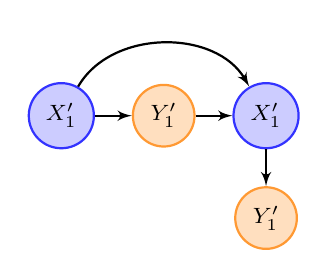
\begin{tikzpicture}[node distance=1.3cm,auto,>=latex']
\node (X_0)   [state] {$X_1'$};
\node (Y_0)   [measurement,right of=X_0] {$Y_{1}'$};
\node (X_1)   [state,right of=Y_0] {$X_1'$};
\node (Y_1)   [measurement,below of=X_1] {$Y_1'$};
%\node (X_1)   [state,above of=X_2] {$X_1'$};
 \path[->] (X_0) edge[thick] (Y_0);
 \path[->] (X_0) edge[thick,style={bend left=60}] (X_1);
 \path[->] (Y_0) edge[thick] (X_1);
 \path[->] (X_1) edge[thick] (Y_1);
% \path[->] (X_2) edge[thick] (Y_2);
 \end{tikzpicture}}
 \caption{Rearrangement of a directed acyclic graph. $X_0'=X_1$, $Y_0'=\{Y_1,Y_3\}$, $X_1'=(X_3,X_2)$ and $Y_1'=\{Y_2,Y_4\}$.}
 \label{fig:graphorder}
 \end{center}
 \end{figure}


\subsection{Sequential Monte Carlo algorithm}
Assume that we have variables $(X,Y)$ which are sorted as described above. By convention, let $x_{a:b}=(x_a,\ldots,x_b)$, $a\leq b$. Sequential Monte Carlo methods~\citep{Doucet2001,DelMoral2004,Doucet2010} proceed by sequentially approximating conditional distributions $\pi_t(x_{0:t}|y_{0:t})$, $t=0,\ldots,n$ by a weighted set of $N$ particles $(x_{0:t}^{(i)},w_t^{(i)})$ that evolve according to two mechanisms
\begin{itemize}
\item \textbf{Mutation/Exploration}: Each particle $i$ is randomly updated from $x_{0:t}^{(i)}$ to $x_{0:t+1}^{(i)}$
\item \textbf{Selection}: Each particle is associated a new weight $w_t^{(i)}$. High weight particles are duplicated while low weight particles are deleted.
\end{itemize}

From the weighted approximation, several statistics (mean, variance, quantiles, etc.) can be extracted on the variables. The vanilla sequential Monte Carlo algorithm is given in Algorithm 1 where `$\sim$' means `statistically distributed from'.

\begin{algorithm}
\caption{Classical Sequential Monte Carlo algorithm}
\label{algo}
$\bullet$ For $t=0,\ldots,n$

$\qquad \bullet$ For $i=1,\ldots,N$, Sample $\widetilde{x}_t^{(i)}\sim q_t$


$\qquad \bullet$ For $i=1,\ldots,N$, set
$$
\widetilde{w}_t^{(i)}\propto\frac{\pi(y_t|\text{pa}(y_t))\pi(\widetilde{x}_t^{(i)}|\text{pa}(\widetilde{x}_t^{(i)}))}{q_t(\widetilde{x}_t^{(i)})}
$$
with $\sum_{i=1}^N \widetilde{w}_t^{(i)}=1$.

$\qquad \bullet$ Duplicate particles of high weight and delete particles of low weight. Let $x_{0:t}^{(i)}$ be the resulting set of particles with weights $\frac{1}{N}$.
\end{algorithm}

$q_t$ is the proposal/importance density function and is used for exploration. Several choices can be made. The simplest is to use the conditional distribution $\pi(x_t|\text{pa}(x_t))$, which is directly given by the statistical model, as a proposal distribution. A better choice is to use the distribution $\pi(x_t|\text{pa}(x_t), y_t)$, or any approximation of this distribution.

\subsection{Particle MCMC}
Shoud we describe this here?

\section{Biips software}
\label{sec:biips}
\subsection{Biips}
\subsection{Rbiips}
\subsection{Matbiips}

\section{Tutorial}
\label{sec:examples}

\subsection{Model and BUGS file}
\lstinputlisting[style=bugs]{../../examples/tutorial/hmm_1d_nonlin.bug}

\subsection{Sequential Monte Carlo}
%\begin{minipage}[l]{0.45\linewidth}
\lstinputlisting[style=matbiips, firstline=171, lastline=193]{../../examples/tutorial/tutorial1.m}
%\end{minipage}
%\begin{minipage}[r]{0.45\linewidth}
\lstinputlisting[style=Rbiips, firstline=1, lastline=20]{../../examples/tutorial/hmm_1d_nonlin.R}
%\end{minipage}

\subsection{PIMH}

\subsection{Sensitivity analysis}

\subsection{PMMH}


\subsection{Adding a user-defined function}






\section{Inference in Switching stochastic volatility models with Biips}
\label{sec:switchingstochasticvolatility}

\lstinputlisting[style=matbiips, firstline=171, lastline=193]{../../examples/stoch_volatility/switch_stoch_volatility.m}

\section{Discussion of related softwares and merits/limits of Biips}
\label{sec:discussion}
BUGS and relatives~\citep{Lunn2000,Lunn2012}, JAGS~\citep{Plummer2003}, Stan~\citep{Stan2013}, SMCTC~\citep{Johansen2009}, LibBi~\citep{Murray2013}.

\section{Conclusion}
\label{sec:conclusion}


\bibliographystyle{jss}
\bibliography{biipsbib}


\end{document}
